\renewcommand{\cleardoublepage}{}
\renewcommand{\clearpage}{}

\section{Fermion Masses in the SM and Quark mixing}

As referenced, given the charges of the fermion and lepton fields we cannot construct a gauge invariant theory with explicit mass terms for fermions. 
%
The mass of these particles are generated through couplings to the Higgs, by the Higgs mechanism. We can write these interactions as,
%
\begin{equation} 
\label{eq:Yukawa2}
\mathcal{L}_{Yuk} = Y^u_{ij} \overline{Q_{L_i}} u_{R_j}  \tilde{H} + Y^d_{ij} \overline{Q_{L_i}}  d_{R_j} H  + Y^e_ij \overline{L_{L_i}}  e_{R_i} H + h.c. 
\end{equation} 
%
where $Y^{e,u,d}$ stand for the Yukawa matrices, these are generic $3\times3$ complex non-dimensional coupling matrices, $H$ is the Higgs field with $\tilde{H}$ retaining it's previous definition, $i,j$ are the standard generation indices, $Q_{L_i}$,are the left handed quark doublets, while $d_R$ and $u_R$ are the corresponding right-handed down and up quark singlets respectively in the weak eigenstate basis. 
%
Has the Higgs field settles into the electroweak VEV Eq.\,\ref{eq:Yukawa2} yields mass terms for the quarks and leptons. 
%
The Higgs mechanism generates the mass for all the fermionic and leptonic particles except for neutrinos, this is due to the SM not containing right handed neutrinos, i.e we can't build terms that would lead to neutrino masses.
% 
The addition of right handed neutrino fields is very commonly made in BSM scenarios. 

To reach the physical states starting from the weak eigenbasis you must diagonalize the Yukawa matrices. This is done through a bi-unitary transformation. 
% 
We can write these transformation under the form,
%
\begin{equation}
\label{YukawaMasses} 
M^{u,d,e}_{\text{diag.}}= U^{u,d,e}_L Y^{u,d,e} U^{u,d,e}_R \frac{v}{\sqrt{2}} 
\end{equation} 
%
where $v$ stands for the electroweak VEV. And $U^{u,d,e}_L$ and $U^{u,d,e}_R$ are the required 6 unitary matrices. 
%
{ \color{blue}
It is, in fact, these matrices that will get us from the flavour eigenbase to the mass eigenbase. } 
%
%{\color{gray} The charged lepton Yukawa matrix can always be made real and positive through a bi-unitarity transformation.  
%
%Meaning the Yukawa matrix for the leptons contains only 3 real physical parameters that correspond to the Lepton masses. } 
%
Naturally we can invert Eq.\,\ref{YukawaMasses}, returning equations for the Yukawa matrices as, 
\begin{align}
\label{eq:YukawaBiUni}
\begin{split}
Y^u_{ij} = & \frac{\sqrt{2}}{v} (U_L^u M^u_{\text{diag.}} U_R^u)_{ij} \\
Y^d_{ij} = & \frac{\sqrt{2}}{v} (U_L^d M^d_{\text{diag.}} U_R^d)_{ij}
\end{split}
\end{align}
%
We can see this change creates mass terms for physical quark fields by replacing the result of eq.\,\ref{eq:YukawaBiUni} in the Yukawa portion of the Lagrangian (Eq.\,\ref{eq:YukawaSM}).
%
\begin{gather}
\mathcal{L}_{Yuk} \supset 
- \frac{v}{\sqrt{2}} Y^d_{ij} \begin{pmatrix} \overline{u}_{L\,i} & \overline{d}_{L\,i}  \end{pmatrix}  d_{R\,j} 
%
-\frac{v}{\sqrt{2}} Y^u_{ij} \begin{pmatrix} \overline{u}_{L\,i} & \overline{d}_{L\,i}  \end{pmatrix} \, u_{R\,j} + h.c. \nonumber  \\ 
% % % 
 \Downarrow \nonumber \\
-(U_L^d m^d_{\text{diag.}} U_R^d)_{ij} d_{L\,i} \, d_{R\,j}  - (U_L^u m^u_{\text{diag.}} U_R^u)_{ij} u_{L\,i} \, u_{R\,j} + \big(\text{Interactions}\big) + h.c \\ 
 \Downarrow  \nonumber \\ 
-m^d_{\text{diag.}_j} d_{L\,i}^\prime \, d_{R\,j}^\prime  - m^u_{\text{diag.}_j} u_{L\,i}^\prime \, u_{R\,j}^\prime + \big(\text{Interactions}\big) + h.c  \nonumber  
\end{gather}
%
where the primed fields are the quark fields in the mass basis, defined as, 
\begin{equation}
\begin{split}
d^\prime_{L,R} = U^d_{L,R} d_{L,R} \\
u^\prime_{L,R} = U^u_{L,R} u_{L,R} 
\end{split}  
\end{equation}
% 
Note that the increasing masses seen in each generation depend directly on the term hierarchy of the Yukawa terms. This means that the mass of all particles directly relate to how strongly they each interact with the Higgs boson.
%
If you then take into account the real masses e.g. for the leptons, the tau mass is in the GeV range while the electron's is in the 0.1 MeV range. These translate to very different couplings for each flavour. 
%
This hierarchy is unjustified in the SM. 

As a result of this redefinition we can now look at the gauge interactions to see that a charge current appears where $W^\pm$ couples the physical $u^\prime_{L_j}$ and $d^\prime_{L_j}$. 
%
The coupling of the of fermions to their respective gauge fields changes by virtue of the fact only left handed Quarks are $SU(2)_L$ doublets, if we expand the up and down quark fields on the kinetic portion of the Lagrangian,
%
\begin{align}
\label{LagFermFCCCs}
\begin{split}
\mathcal{L}_{ferm} \supset & 
\frac{1}{2} \overline{u^\prime_L} \gamma^\mu \left( g^\prime Y_L B_\mu + g W^0_\mu  \right) \left(U^u_L U^{u \dagger}_L \right) u^\prime_L - \frac{1}{\sqrt{2}} g \overline{u^\prime_L} \gamma^\mu \left( U^u_L U^{d \dagger}_L \right) d^\prime_L W^+_\mu \\ \nonumber   
- 
& \frac{1}{\sqrt{2}} g d^\prime_L \gamma^\mu \left( U^u_L U^{d \dagger}_L \right) u^\prime_L W^-_\mu 
+ 
\frac{1}{2} \overline{d^\prime_L} \gamma^\mu \left( g^\prime Y_L B_\mu - g W^0_\mu \right) \left( U^d_L U^{d \dagger}_L \right) d^\prime_L  
\end{split}
\end{align}
%
We can trough the use of the properties of unitary matrices, namely, $ \mathrm{U}^{u,d}_{L,R} \mathrm{U}^{u,d \dagger}_{L,R} = 1$, note that the interactions with the neutral bosons remain the same in the mass basis.
%
However the charged currents are affected by this change.
%
There for, we define the Cabibbo-Kobayashi-Maskawa (CKM) matrix, as $V_{CKM} = U^u_L U^{u ^\dagger }_R $ and write the sensitive terms,
%
\begin{equation}
\mathcal{L}_{kin} \supset \frac{1}{\sqrt{2}} g \overline{u}^\prime_L \gamma^\mu V_{CKM} d_L^\prime W^+_\mu + h.c. 
\end{equation}
%
The CKM matrix, is a $3 \times 3$ unitary matrix. It is a parametrization of the three mixing angles and CP-violating KM phase. There are many possible conventions to represent the CKM matrix.
%
The mixing angles refer to those between the up and down quark families. We can see their hierarchy in Fig. \ref{fig:QuarkCKM}.

It is through this complex phase in the CKM matrix that the SM can account for the phenomena of $\mathcal{CP}$ violation. First observed in the famous $K^0$ decay into $\mu^+$ $\mu^-$ ($CP=+1$ and $CP=-1$ respectively) that won the 1980 Nobel Prize. The discovery opened the door to questions still at the core of particle physics and of cosmology today. Not just the lack of an exact CP-symmetry, but also the fact that it is so close to a symmetry. {\color{blue} citation}

\begin{figure}[H]
	\centering
	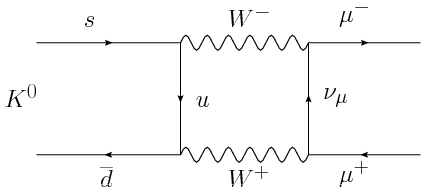
\includegraphics[width=0.5\textwidth]{Glashow-Illiopoulos-Maiani_mechanism_fig1.png}
	\caption{Box diagram describing $K_L^0\rightarrow\mu^-\mu^+$, through an intermediate $u$ quark.}
	\label{fig:Kaon}
\end{figure}

We avoided discussing leptons since in the SM their mass eigenstates can be easily shown to have no real consequence besides a change of basis. 
%
You might also note a very interesting feature of the Standard Model, by consequence of the $\mathrm{SU(2)_L \times U(1)_Y }$ symmetry there are no interactions of the right handed unitary matrices and there for no mixing, coupling, or charged currents of right handed quarks, making them theoretically invisible to measurements.  
%
\begin{figure}[H]
	\centering
	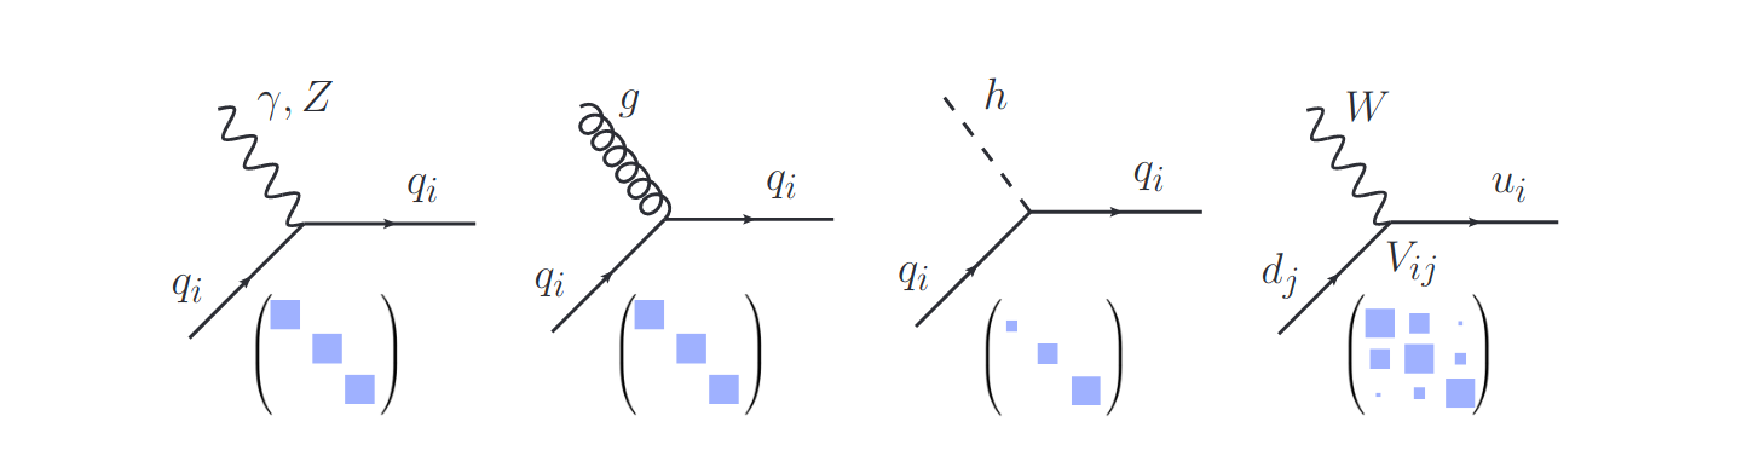
\includegraphics[width=0.9\textwidth]{TestYukawaCouplings.pdf}
	\caption{The Feynman diagrams for flavour conserving couplings of quarks to photon, $Z$ boson, gluon and the Higgs (the first three diagrams), and the flavour changing coupling to the $W$ (the last diagram). The $3\times3$ matrices are visual representations of couplings in the generation space, with couplings to $\gamma$ ,$Z$, $g$ flavour universal, the couplings to the Higgs flavour diagonal but not universal, and the couplings to $W$ flavour changing and hierarchical.}
	\label{fig:QuarkCKM}
\end{figure}
%

% Possible power gap
%
% Here we introduce the CKM matrix, a $3 \times 3$ unitary matrix. It is a paramatrization of the three mixing angles and CP-violating KM phase. There are many possible conventions to represent the CKM matrix. 

The CKM matrix elements are fundamental parameters of the particle physics, so their precise determination is important, and reproducing the quark mixing parameters is fundamental for BSM searches that include changes to how the quarks interact with possible new Higgs bosons. 
